\documentclass[tikz]{standalone}

\usetikzlibrary{automata}

\begin{document}
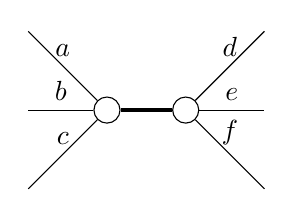
\begin{tikzpicture}
\tikzstyle{vertex}=[draw,shape=circle]
\path (0,0) node[vertex](x1){} (1,0) node[vertex](y1){};
\draw[line width=1.5pt] (x1) -- (y1);
\draw[] (-1,1) -- node[above] {$a$} (x1);
\draw[] (-1,0) -- node[above] {$b$} (x1);
\draw[] (-1,-1) -- node[above] {$c$} (x1);
\draw[] (y1) -- node[above] {$d$} (2,1);
\draw[] (y1) -- node[above] {$e$} (2,0);
\draw[] (y1) -- node[above] {$f$} (2,-1);
\end{tikzpicture}
\end{document}